\chapter{Related Work}
\label{related_work}
Motion planning is a widely researched topic with roots in control, artificial intelligence, computational geometry and Robotics. The literature presented in \cite{book_robot_motion_planning}, \cite{book_lavelle_planning} review significant portion of standard planning techniques. Due to the complexity of the autonomous cars and the environments, general techniques from robotics cannot be applied. Planning for autonomous cars, in general, is subdivided into two categories namely planning in unstructured environments such as parking areas etc and structured environments such as Road Networks where the traffic rules have to be followed. This chapter mainly focuses on the planning techniques in structured urban environments. The following subsections discuss regarding various approaches involved in planning, path representation techniques and finally regarding trajectory evaluation. 

\section{Planning Approaches}
\label{planning_aproaches}

Autonomous vehicles have been in research communities from 80's with projects such as PROMETHEUS \cite{prometheus}, the research was accelerated by competitions such as DARPA Grand Challenge in 2006 and DARPA Urban Challenge(DUC) in 2007 \cite{darpa_urban_challenge}. In DUC, six autonomous vehicles from different universities have completed the challenge and have used various techniques to accomplish the task. The methods developed during these events formed the basis for modern-day autonomous cars which perform with greater safety and comfort compared to the DUC participants. 

Approaches followed by different participants of DUC are described in \cite{darpa_urban_challenge}. All these participants follow a similar approach with differences in internal techniques to solve subproblems. Planning module of Boss, autonomous vehicle from Carnegie Melon University which won the DUC is described in general here. Its planning framework is mainly subdivided into 3 submodules 

\begin{itemize}
	\item Mission control: It is the higher level module which creates a global path, assigns lane to the vehicle to reach the checkpoints and detects blockades.
	\item Behavioral module: It is responsible for decisions such as precedence at intersections, lane change decision, speed planning, look ahead point assignment etc. 
	\item Motion planning module: It is responsible for generating local trajectories and converting them to steering and acceleration values. It initially creates a forward looking path and velocity planning is performed on top of that. 
\end{itemize}

After DUC, research efforts have been increased to develop state of the art solutions in perception, planning and control of autonomous vehicles. Motion planning plays a crucial role in the system with aim of building trajectories that are collision free and also adhere to kinematic and dynamic constraints of vehicle, road boundaries and traffic rules \cite{motion_planning_techniques}. There have been numerous approaches to solving the problem of path planning and some of them are discussed in this section. Potential fields is one of such algorithm, it models state space as with attractive forces towards goal and repulsive near obstacles \cite{potential_field_3} \cite{potential_field_1} \cite{potential_field_2}. In this approach path is found by travelling along the steepest gradient of the potential field, however, there is a risk of paths getting trapped in local minima. Grid-based approach is another generally used method in Robotics, here environment is perceived as a set of grids and path is found travelling across these grids using algorithms like A*. The downside of these approaches is that the complexity increases exponentially with increase in grid resolution and grid size, there have been different variants of this approach as discussed in \cite{A_star} \cite{D_star_1} \cite{kolski_thesis}. A comprehensive study of various approaches in motion planning for autonomous vehicles is presented in \cite{motion_planning_techniques} \cite{survey_planning_techniques}.

 Planning approaches that are widely used in autonomous driving are classified as shown in Figure \ref{related_work_classification}. The following subsections discuss research in each of the described categories. 

\begin{figure}[H]
	\centering
	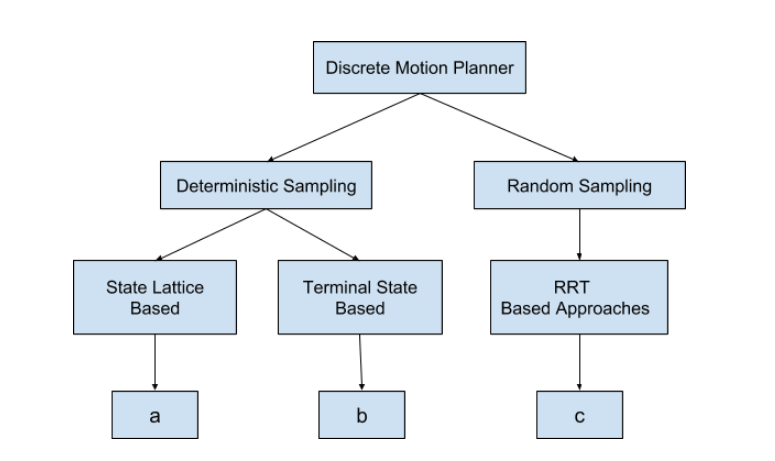
\includegraphics[width=0.8\textwidth]{Images/related_work/planning_division.png}
	\caption{General Overview of On-road planners. a - \cite{cmu_parallel_thesis}  \cite{diss_shui_phd_thesis} \cite{traj_planner_optimization} \cite{lattice_Gu_Tiyanu} \cite{unit_A_star} , b - \cite{kolski_thesis} \cite{real_time_traj_plan_article} \cite{darpa_urban_challenge}, c -\cite{rrt_star} \cite{rrt_urban_driv} \cite{mit_rrt}
	}
	\label{related_work_classification}
\end{figure}
\todo{change terminal state to local search}

\subsection{Random Sampling Approaches}
\label{rw_incremental_search}
Rapidly-exploring Random Tree(RRT) technique was initially introduced by Steven M. LaValle in his work presented in \cite{Lavalle_rrt}. RRT builds a tree incrementally by sampling new states. In each iteration, a new sample $x$ is sampled and connected to the nearest neighbour $x_\textsubscript{neartest}$ in the tree if it is collision free. The tree starts at the start location and is built till the path to goal location is found. Probabilistic Roadmaps algorithm\cite{prm}(PRM) is another approach where uniform sampling is performed across the state space and are connected if a collision-free path exists. Then a graph search algorithm is employed to find a path from source to destination. Both of these approaches are probabilistic complete, i.e., as the number of samples increases the probability of finding a solution approaches 1 given problem is solvable.


Different variants of RRT's are widely accepted in robot motion planning because of its ability to explore higher dimensional problems at ease\cite{rrt_higher_dimension}. To improve the performance of RRT, bidirectional RRT with two trees(Bi-RRT) has been proposed, though it improves the performance, handling discontinuities of two trees is difficult\cite{birrt}. Environmentally guided RRT(EG-RRT) is another variant that incorporates information from scene analysis has been applied in real-world scenarios\cite{egrrt}. MIT has applied a closed loop prediction model into RRT(CL-RRT) in its autonomous vehicle at DUC \cite{mit_rrt}, a snippet of planning is shown in Figure \ref{mit_rrt_fig}. In CL-RRT motion models are used to generate trajectories to sampled states and are evaluated for feasibility and performance. A variant named RRT* \cite{rrt_star} has been proposed which guarantee asymptotic optimality. In this approach, each state stores cost from start and when a new sample is added, surrounding neighbours are tested if a better path can be found and the tree is rewired thus leading to an efficient path. There have been many techniques to reduce the number of sampled states in-order to save computational time, Informed-RRT \cite{informed_rrt} is one such approach which samples space according to the actual best path and states that are far away from the goal are not sampled.

\begin{figure}
	\centering
	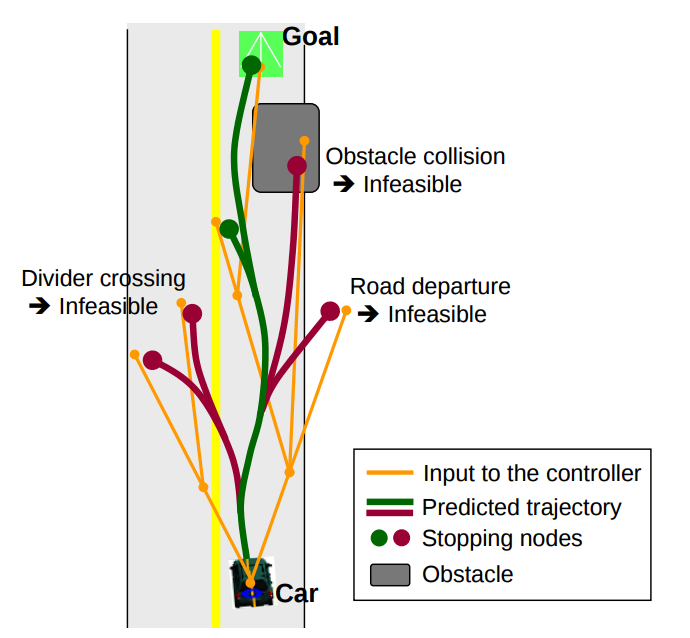
\includegraphics[width=0.6\textwidth]{Images/related_work/mit_urban_planning.png}
	\caption{MIT Darpa Urban Challenge - RRT based planning approach}
	\label{mit_rrt_fig}
\end{figure} 

In real-world situations' environment is not completely predictable and the computed path needs to be dynamically re-planned over the time. This needs either a new plan to be generated quickly or rapid correction of old path. The approach Anytime-RRT \cite{anytimerrt} creates an initial path using RRT and optimizes it on the go to create an optimal path, re-planning is triggered when the path is no longer valid. The method RRT$^x$ \cite{rrtx} updates the search space whenever obstacle changes are observed and repair the surrounding tree. 

Though RRTs are best-performing algorithms in planning, they exhibit certain deficiencies in terms of motion planning for autonomous vehicles, especially in on-road driving conditions. RRT-based planners generate jerky and unnatural trajectories that contain many unnecessary turns\cite{improved_rrt}, these are suitable for open areas such as parking areas. Road parallel trajectories are preferred in structured environments.

\subsection{Lattice Planners}
\label{rw_lattice_planners}
The lattice planners use a discrete representation of the planning area with multiple states, often multi dimensional one with dimensions such as position, acceleration, velocity, time, curvature, heading etc. These states are connected together and the problem then reduces to finding a path from the initial state to the final state in the lattice. This approach is generally well suited for non-holonomic robots and highly constrained areas such as road networks\cite{lattice_1}. Lattice planners are resolution complete, i.e., they can be automatically adjusted to change in resolution to explore state space consistently. The approach proposed in \cite{lattice_1} uses a multi-resolution state lattice with high resolution near start and goal locations and lower resolution in middle to reduce computational complexity. Continuity of path and curvature are constraints in path planning, these are addressed in the research \cite{lattice_2} by defining a 4D configuration including 2D position, heading and steering. In \cite{cmu_parallel_thesis} the author added curvature to each state along with 2D position heading and curvature, paths between the vehicle and sampled sates are connected using third order spirals. A range of times and velocities are assigned to each vertex to enable spatiotemporal search. It uses constant acceleration profiles are chosen making it difficult for the vehicle to follow. Thus, due to a multitude of states involved the number of trajectories created are in order of few hundred thousands and increase exponentially if the resolution is increased or new dimension is added. A graphical processing unit(GPU) is needed to run the evaluations in parallel to provide real-time response. 

To improve the performance of \cite{cmu_parallel_thesis}, the research published in \cite{traj_planner_optimization} utilizes quartic polynomials to ensure continuous curvature, connections are made from sampled endpoints and current state, Figure \ref{trajopt} shows further information about path and velocity representation. In this approach, speed profiles are generated inversely and checks are included to ensure comfort, efficiency. To reduce the computational complexity the approach proposed in \cite{traj_smoothing} uses a two-level planning approach which initially generates optimal collision-free reference path and then performs the search across this reference path to find an optimal trajectory. The reference path leads to a focused search and more human-like driving style. The research published in \cite{diss_shui_phd_thesis} further improves the trajectory smoothness ensuring a high level of trajectory diversity.

In summary lattice planners create trajectories that are smooth, optimal and complying with dynamic and kinematic constraints of the vehicle. These approaches are well suited for structured and dynamic environments. They are also computationally expensive and complexity increases exponentially with the addition of new state or increase in resolution.

\begin{figure}
	\centering
	\begin{subfigure}{.52\textwidth}
		\centering
		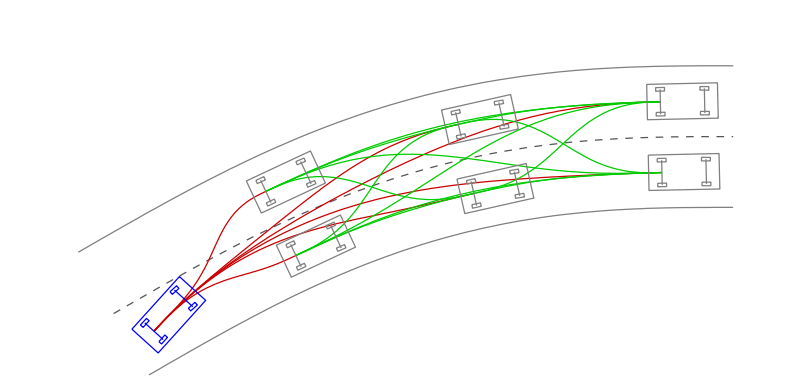
\includegraphics[width=1.0\linewidth]{Images/related_work/traj_optim_1.png}
		\caption{Path set. blue vehicle - current vehicle pose, and grey vehicles - sampled endpoints, red paths-quartic curvature polynomials and green paths - cubic ones}
		\label{trajoptsub1}
	\end{subfigure}%
	\begin{subfigure}{.48\textwidth}
		\centering
		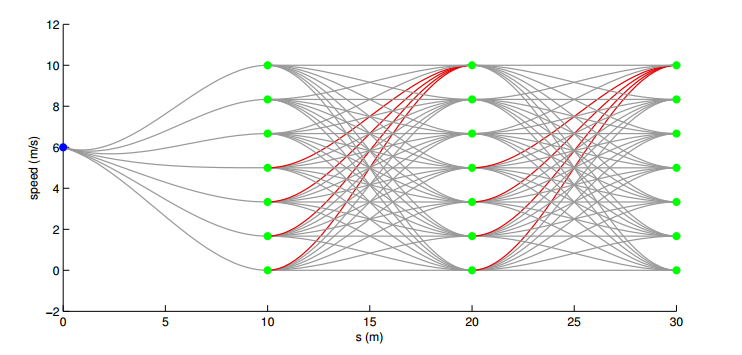
\includegraphics[width=1.0\linewidth]{Images/related_work/traj_optim_2.png}
		\caption{Speed set. The green points are sampled speeds, the
red curves are beyond the acceleration limit, and the grey
curves are valid ones}
		\label{trajoptsub2}
	\end{subfigure}
	\caption{Path velocity representation in \cite{traj_planner_optimization}}
	\label{trajopt}
\end{figure}

\subsection{Local Search}
\label{rw_local_search}

Local search is the most popular technique in autonomous driving, in this method instead of searching the complete graph a local state space is searched for a feasible solution as shown in \ref{cmubossduc}. The planners proposed in \cite{darpa_urban_challenge} \cite{juniorstanford} \cite{kolski_thesis} \cite{Broggi2012} \cite{real_time_traj_plan_article} \cite{urbansafetyeth} perform some format of local search. The generated candidate trajectories are evaluated with a set of cost functions for collision checking and comfort to finalize the final trajectory. Paths with lateral shifts can generally be split into two categories i.e., lateral shifts in action space(controls as a function of time and controls as a function of time and state) and state space(position, orientation, linear and angular velocities, curvature) of vehicle\cite{howard_phd}. Partial motion planning is another technique used to search locally reducing computational power significantly \cite{partialmotionplanning}. In summary, local search algorithms can create short-term trajectories at a low computational cost with limitations in the manoeuvres robot can perform, these are especially suitable for low-speed and on-road driving.

\begin{figure}
	\centering
	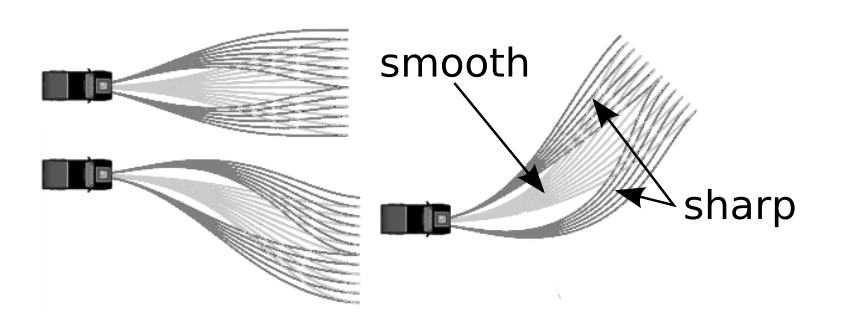
\includegraphics[width=0.6\textwidth]{Images/related_work/trajectorysetbossduc.png}
	\caption{CMU Darpa Urban Challenge - Local Search Forward projected trajectories}
	\label{cmubossduc}
\end{figure} 

\section{Trajectory Representation}
\label{trajrep}
Trajectory or path representation is another important factor in quantifying the trajectories, there are different methods such as arcs, second to fifth order polynomials, Cubic to Quintic Bezier curves, Dubian Paths, Reeds-Shepp curves, Akima splines, splines etc. Each of these curves has different advantages, disadvantages and suitable in different environments as discussed in \cite{motion_planning_techniques}. Splines and polynomials are used for creating road parallel trajectories, fifth order polynomials produce jerk minimizing trajectories\cite{werling_frenet} and other formats are also employed by different planners. Reeds-shepp curves, a version of Dubian curves allow forward and backward driving \cite{reedsshepp} thus making them suitable for complex manoeuvres in parking lots, obstacle course etc.


\section{Trajectory Evaluation}
\label{traj_eval}
Trajectory created by different methods mentioned in previous sections must be validated against various constraints to check feasibility, comfort, optimality and collision. \cite{traj_planner_optimization} uses cost functions to check each trajectory for path length, curvature, the rate of change of curvature, lateral offset to the closest centre line, transformed distance to static obstacles, duration of the plan, speed, acceleration, jerk, centripetal acceleration, distance to dynamic obstacles. All the planners' test for some or all of the parameters mentioned using cost functions, some weigh each cost differently based on optimizing factor, \cite{unit_A_star} penalize breaking to prefer long-range trajectories, \cite{cmu_parallel_thesis} penalizes shorter horizons to ensure minimum horizon. Major criteria for trajectory evaluation is collision checking to ensure safe motion.

Simulation-based techniques are widely used in collision checking where the vehicle is simulated in time to check for collision with other obstacles.

In \cite{kolski_thesis}, for collision checking in static environments map is represented as grid cells and based on obstacles and traversable areas the cells are assigned cost and the trajectories that pass through these cells are added with corresponding costs. In dynamic environments' vehicle shape is forwarded and checked for collision with static obstacles as represented in Figure \ref{kolskicollison}.
\begin{figure}
	\centering
	\begin{subfigure}{.50\textwidth}
		\centering
		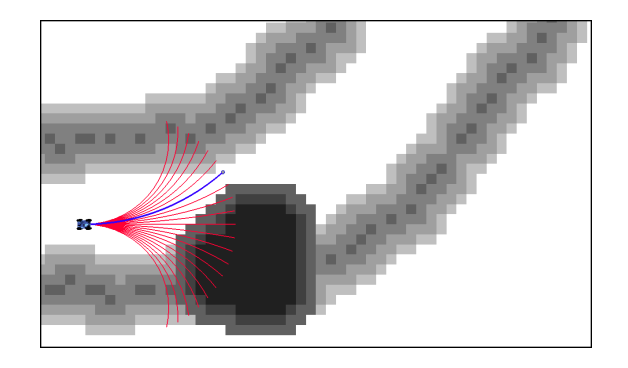
\includegraphics[width=1.0\linewidth]{Images/related_work/kolskistaticobst.png}
		\caption{Static Environments - Cost of path is computed based on cost of the cells it traverses through, darker the cell higher the cost.}
		\label{kolski1}
	\end{subfigure}%
	\begin{subfigure}{.50\textwidth}
		\centering
		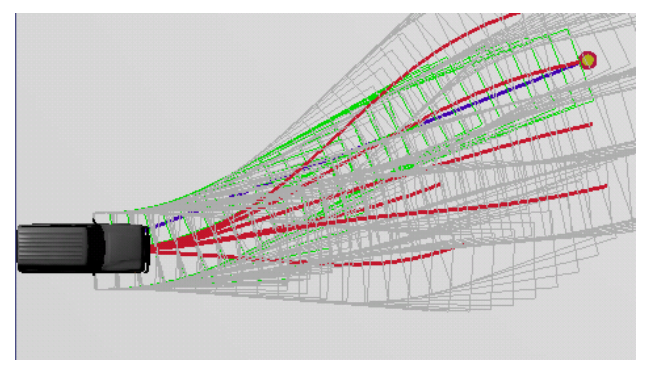
\includegraphics[width=1.0\linewidth]{Images/related_work/dynamiccollsionkolski.png}
		\caption{Dynamic Environments, Static Obstacles- For series of trajectories vehicle shape is forwarded and collision checking is performed}
		\label{kolski2}
	\end{subfigure}
	\caption{Collision Checking \cite{kolski_thesis}}
	\label{kolskicollison}
\end{figure}

For collision checking with dynamic obstacles, \cite{kolski_thesis} uses a hierarchical approach. In this method initially given vehicle trajectory and obstacle trajectory bounding boxes are constructed and checked for collision, if they intersect then in incremental time steps a pessimistic approximation of circles is used to check for collision, if they also collide then actual model of the car is used to check for collision as represented in Figure \ref{kolskidynamicobst}.

\begin{figure}
	\centering
	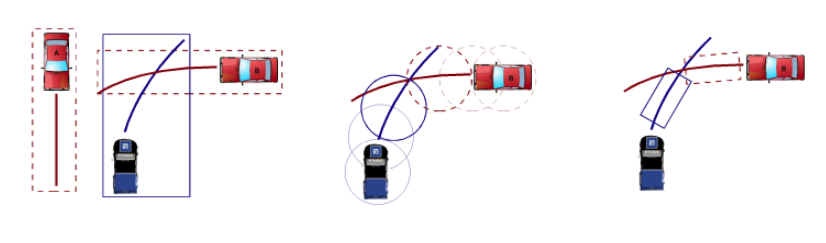
\includegraphics[width=1.0\textwidth]{Images/related_work/kolskidynamicobstacles.png}
	\caption{Collison checking for Dynamic Obstacles \cite{kolski_thesis}}
	\label{kolskidynamicobst}
\end{figure} 

In \cite{cmu_parallel_thesis}, for collision checking with respect to static obstacles each (x,y) point in world is assigned a cost based on proximity to static obstacles, a path that intersects with obstacles has lethal cost, paths that have close proximity to these obstacles have high costs and paths that are away from obstacles are assigned zero cost. A Potential function is created based on the position of obstacles to that computes the cost of the path. Similarly, for dynamic obstacles, a potential function is created by adding t dimension to create cost function in (x,y,t). Static and dynamic obstacles are dilated accordingly to remove errors in perception and ensure safety.


In \cite{rrt_star} collision checking is performed by forward predicting the vehicle shape represented as rectangle and collision checking with lines joining the initial and final state of obstacles and border lines. The planner proposed in \cite{volvo_reactive_traj} presents a reactive approach, in this distance to the dynamic obstacles ahead, is used as a parameter to stop the vehicle.

The approaches proposed for collision checking rely on predicting future trajectory by assumptions that obstacles will continue with constant velocity, acceleration, current orientation, in the same lane etc., these assumptions are not accurate and may lead to inefficiencies due to ignoring traffic context, interactions between vehicles etc \cite{motion_planning_techniques}. There are also uncertainties in data predicted by the perception module, and they must be considered while collision checking.

In summary, collision checking is an important and also a complex task which involves different types of checks, assumptions, and approximations to create trajectories that are safe.


\todo{summary of complete related work}

%Look if the sampling based, RRT based, lattice based etc etc should be combined together?
%write about MDP, POMDP etc 